%%%%%%%%%%%%%%%%%%%%
%% KAPITEL Intro %%
%%%%%%%%%%%%%%%%%%%
\section{Einführung}
% MARCO
% was ist es, wer benutzt es, wofür braucht man es
% erreichbar durch Transaktion SWDD, im SAP System eingebaut usw
%%%%%%%%%%%%%%%%%%%%%%%%%%%%%%%%%%%%%%%%%%%%%%%%%%%%%%%%%%%%%%%%%
% http://www.connexin.net/de/sap-transaktionen-uebersicht.html
% -> Hier auch die Workflow transaktionen mit LOG etc erwähnen!
% http://help.sap.com/saphelp_nw04s/helpdata/EN/c5/e4b79d453d11d189430000e829fbbd/content.htm
% -> Bild zum Beispiel für die Übersicht des Builders zu erklären
% http://www.sdn.sap.com/irj/scn/go/portal/prtroot/docs/library/uuid/3c2b9c90-0201-0010-ab86-a574c7881607?QuickLink=index&overridelayout=true&5003637211723
% -> schöne Definitionen und Übersicht des Builders
% http://www.edv-buchversand.de/sap/chapter.php?cnt=getchapter&id=gp-9285.pdf
% -> auch sehr gut für Übersicht!!
% http://www.abap-tutorials.com/wp-content/uploads/pdfs/workflow_tutorial.pdf
% -> geil für die Einführung mit Warum brauchen wir überhaupt Workflows etc..
\subsection{Warum ein SAP Workflow Builder?}
\label{sec:warum-wf-builder}
Durch eine sehr breite Produktpalette und lange Erfahrung ist in einem \gls{sap} System standardmäßig eine sehr große Menge an Arbeitsabläufen vorhanden und direkt einsetzbar. Aufgrund der Verschiedenheit individueller Firmen und Branchen ist es allerdings unmöglich, alle möglichen Workflows zu integrieren und zur Verfügung zu stellen. Daher stellt die \gls{sap} ihren Kunden unter dem \gls{transaktionscode} \texttt{SWDD} eine Möglichkeit zur Verfügung, mit der sie, nach einer gewissen Einarbeitungszeit, beliebige Workflows selbst abbilden können. Dadurch können gekaufte Produkte mit einer maximalen Genauigkeit in die vorhandenen Betriebsabläufe integriert und auch schon vorhandene Fremdsysteme angesprochen werden \cite{SAPHelpWf}.

\subsubsection{Vorteile des SAP Workflow Builders}
\label{sec:vorteile-sap-wf-builder}
Durch die direkte Einbindung in das \gls{sap} System hat der Workflow Builder einige Möglich\-keiten und Funktionen, die mit einem externen Programm nicht umsetzbar wären. So ist es möglich, auf interne Ereignisse zu warten und auf diese zu reagieren. Des weiteren können auch globale Ereignisse ausgelöst werden und es kann problemlos mit anderen \glspl{transaktion} des Systems zusammengearbeitet werden. 

Da viele Firmen zur Verwaltung der Produktion, des Personals und anderen Dingen größtenteils \gls{sap} Systeme im Einsatz haben, ist es somit möglich, ein Maximum an Automatisierung zu erreichen.

\subsection{Programmoberfläche}
\label{sec:win-overwiev}
Die Programmoberfläche des Workflow Builders (Abbildung \ref{abb:workflow-overview}) ist in verschiedene Bereiche unterteilt. Die wichtigsten sind die im Folgenden beschriebenen.

\begin{figure}[h]
	\begin{center}
	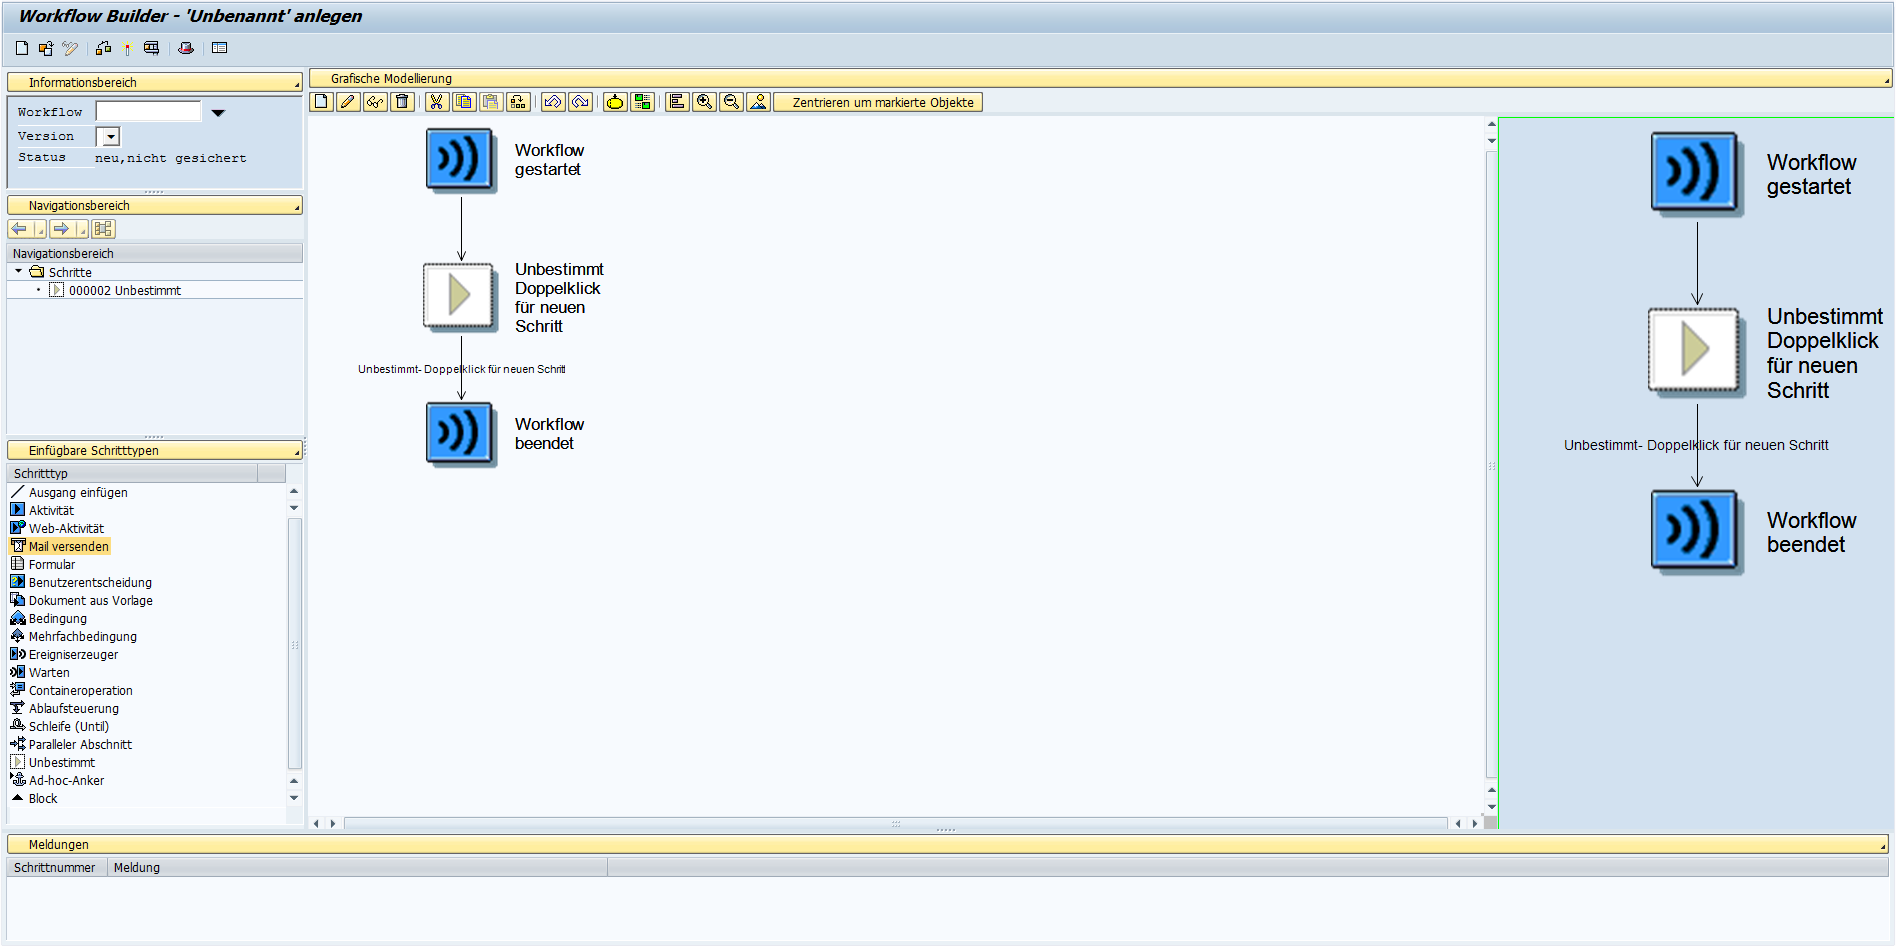
\includegraphics[width=1.0\textwidth]{grafiken/wf-builder_overview.png}
	\caption{Programmübersicht: Der SAP Workflow Builder}
	\vspace{-10pt}
	\label{abb:workflow-overview}
	\end{center}
\end{figure}

\subsubsection{Workflow}
\label{sec:win-overview-wf}
Dieser Bereich ist der wichtigste und größte. Hier wird der Bereich des modellierten Arbeitsablaufs, der gerade bearbeitet wird, groß dargestellt und es können neue Schritte eingefügt werden, vorhandene Schritte editiert oder gelöscht werden. Ein Doppelklick auf einen Schritt bringt den Benutzer zur gespeicherten Definition des Elements, welche dort gepflegt werden kann.

\subsubsection{Übersicht}
\label{sec:win-overview-uebersicht}
Die grafische Übersicht bietet dem Bearbeiter stets einen Überblick des gesamten Workflows, wofür dieser bei großen Modellierungen stark verkleinert dargestellt werden muss. Zusätzlich signalisiert ein grüner rechteckiger Rahmen stets, welcher Teil des Gesamtbildes aktuell im großen Workflow Fenster bearbeitet wird. Durch Verschieben des Rahmens ist es möglich, direkt zu einem gewünschten Teil zu springen.

\subsubsection{Schritttypen}
\label{sec:win-overview-schrittypen}
Der untere linke Bereich des Programms hat standardmäßig den Titel "`Einfügbare Schrittypen"' und enthält eine Liste aller Schrittypen, die verwendet werden können. Von hier können diese mit der Maus per \gls{dragdrop} in den Prozess eingefügt werden. Beim Einfügen des Schrittes wird durch ein kleines Plus am Mauszeiger signalisiert, dass der entsprechende Schritt an dieser Stelle eingefügt werden kann.

\subsubsection{Informationsbereich}
\label{sec:win-overview-information}
Der Informationsbereich zeigt an, welcher Workflow aktuell geladen ist, dessen Status und Versionsnummer. Durch einen Klick auf die Auswahlliste neben "`Version"' kann eine andere Version des gespeicherten Prozesses geladen werden. Um einen neuen Prozess zu laden, kann entweder, wenn diese bekannt ist, die entsprechende Identifikationsnummer in das Textfeld neben "`Workflow"' eingegeben werden oder die Suchhilfe mittels des kleinen Pfeils daneben geöffnet werden. Letzteres öffnet das in Abbildung \ref{abb:workflow-search} gezeigte Fenster, in welchem die auf dem System vorhandenen Workflows nach Kategorien aufgegliedert angezeigt werden.

\begin{figure}[h]
	\begin{center}
	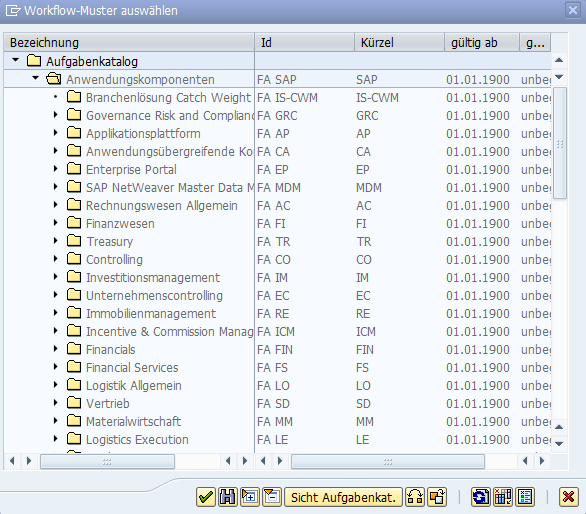
\includegraphics[width=300px]{grafiken/wf-builder_search.png}
	\caption{Suchhilfe des Workflow Builders}
	\vspace{-10pt}
	\label{abb:workflow-search}
	\end{center}
\end{figure}

\subsubsection{Navigationsbereich}
\label{sec:win-overview-information}
Der Navigationsbereich beinhaltet eine Liste aller im Prozess vorhandenen Schritte. Von hier aus ist es möglich, direkt zu der Definition eines gewünschten Schrittes zu springen. 

\subsubsection{Meldungen}
\label{sec:win-overview-meldungen}
In diesem Bereich werden Nachrichten zur Information des Benutzers angezeigt. Dies können allgemeine Benachrichtigungen, Ergebnisse der Syntaxprüfung oder Suchergebnisse sein.

\subsubsection{Alternative Inhalte}
\label{sec:win-overview-alternative}
Zusätzlich zu den standardmäßig beim Programmstart und in Abbildung \ref{abb:workflow-overview} angezeigten Informationen kann die Ansicht \nameref{sec:win-overview-schrittypen} zu einer alternativen Ansicht geändert werden. Dies erfolgt, indem der Benutzer auf die Überschrift "`Einfügbare Schritttypen"' des Bereichs klickt. Aus dem nun geöffneten Menü (Abbildung \ref{abb:workflow-alternatives}) ist einer der Einträge auszuwählen. Die folgenden Ansichten stehen zur Verfügung:

\begin{figure}[h]
	\begin{center}
	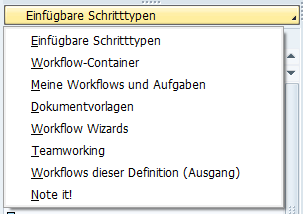
\includegraphics[width=220px]{grafiken/wf-builder_alternative-inhalte.png}
	\caption{Alternative Anzeigemöglichkeiten des Workflow Builders}
	\vspace{-10pt}
	\label{abb:workflow-alternatives}
	\end{center}
\end{figure}

\begin{enumerate}
	\item Der \textbf{Workflow Container} beinhaltet alle Elemente, wie Variablen und Benutzereingaben, welche während der Ausführung des Workflows benötigt werden. Neben den automatisch generierten Container Elementen können auch vom Benutzer definierte Elemente angelegt werden.
	\item Die Ansicht \textbf{Meine Workflows und Aufgaben} bietet einen Schnellzugriff auf alle Workflows, die in letzter Zeit bearbeitet wurden. Des weiteren kann eine eigene Liste an Aufgaben und Workflows angelegt werden.
	\item \textbf{Dokumentvorlagen} sind Dokumente externer Programme (Excel-Tabellen, Word-Dateien oder beliebige andere), welche im Schritt "`Dokument aus Vorlage"' eingebunden werden können. 
	\item \textbf{Workflow Wizards} bieten dem Benutzer die Möglichkeit, häufig genutzte Prozessteile mit Hilfe eines von \gls{sap} bereitgestellten \gls{wizard}s einzufügen.
	\item In der Ansicht \textbf{Teamworking} kann nach Schritten gesucht werden, welche von einer bestimmten Person als letztes bearbeitet wurden.
	\item Der Punkt \textbf{Workflows dieser Definition (Ausgang)} zeigt alle zur Zeit auf dem System ausgeführten Instanzen dieser Workflow Version.
	\item Der letzte Punkt, \textbf{Note it!} bietet dem Benutzer die Möglichkeit, sich Notizen zu seiner aktuellen Arbeit zu erstellen.
\end{enumerate}

\subsection{Funktionen des Builders}
\label{sec:builder-funktionen}
% MARCO
% welche Funktionalitäten hat der Builder...
Im Folgenden sollen nun zuerst die wichtigsten Funktionen des \gls{sap} Workflow Builders erklärt werden. Danach folgt im Kapitel \nameref{sec:builder-elemente} eine breiter gefächerte tabellarische Übersicht. Dort sind auch die Symbole der Schrittypen mit aufgeführt. 

Beim ersten Start des Programms wird dem Benutzer statt einer leeren Arbeitsfläche der minimale Aufbau eines Workflows im \gls{sap}-System angezeigt (Abbildung \ref{abb:workflow-easy}). Dieser besteht aus dem Startereignis "`Workflow gestartet"' und dem Endereignis "`Workflow beendet"'. Dazwischen können beliebige Schritte an Stelle des unbekannten Schrittes (gekennzeichnet durch einen Pfeil auf weißem Hintergrund) eingefügt werden.

\begin{figure}[h]
	\begin{center}
	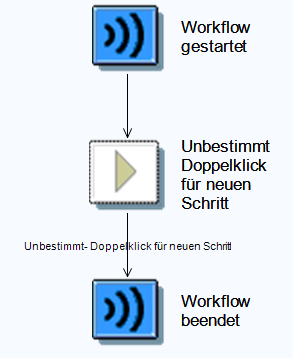
\includegraphics[width=150px]{grafiken/wf-builder_new-wf.png}
	\caption{Initialer Workflow des Builders}
	\vspace{-10pt}
	\label{abb:workflow-easy}
	\end{center}
\end{figure}

\subsubsection{Aktivität}
Der wichtigste Schritttyp ist die Aktivität, welche verschiedene Aufgaben erfüllen kann. Der Benutzer kann entweder einen \gls{abap} \gls{objekttyp} und eine zugehörige Methode oder eine im System vorhandene und schon definierte Aufgabe auswählen. Die entsprechende Aktivität wird dann vom System automatisch gestartet, wenn die Stelle im laufenden Workflow erreicht wird \cite{SAPHelpWf}.

\subsubsection{Web-Aktivität}
Mit Hilfe dieses Schrittes wird aus dem internen Workflow heraus ein \gls{xml}-Dokument an eine URL gesendet. Der Empfänger kann beispielsweise ein anderes System sein, welches daraufhin einen eigenen Workflow startet. Alle \gls{sap}-Systeme stellen einen Service zur Verfügung, welcher in diesem Fall automatisch einen weiteren Workflow starten kann \cite{SAPHelpWf}.

\subsubsection{Mail versenden}
Dieser Schritt versendet eine Nachricht innerhalb des \gls{sap}-Systems. Der Empfänger (es sind mehrere Empfänger möglich) kann diese im internen Postfach abrufen. Der Text der Mail wird bei der Definition des Schrittes festgelegt, wobei Variablen verwendet werden können, welche zur Laufzeit mit den entsprechenden Werten gefüllt werden \cite{SAPHelpWf}.

\subsubsection{Formular}
Ein Formular kann innerhalb des Workflows zur Anzeige von Daten oder deren Bearbeitung durch den Endnutzer verwendet werden. Nachdem bei der Definition des Schrittes die zu bearbeitenden Daten angegeben wurden, erzeugt das Workflow-System automatisch das zugehörige Formular, welches noch bearbeitet werden kann \cite{SAPHelpWf}. 

\subsubsection{Benutzerentscheidung}
Eine Benutzerentscheidung kann mit einem Text versehen werden, welcher dem Endnutzer erklärt, welche Entscheidung er treffen muss. Der Workflow kann so konfiguriert werden, dass er, je nachdem welche der vorgegebenen Antwortmöglichkeiten ausgewählt wurde, einen anderen Pfad wählt \cite{SAPHelpWf}.

\subsubsection{Bedingungen}
Die Schritte Bedingung und Mehrfachbedingung bestimmen, ähnlich der Benutzerentscheidung, den weiteren Ablauf des Workflows. Der Unterschied besteht darin, dass das System die Entscheidung eigenständig nach vorgegebenen Bedingungen fällt und der Benutzer keinen Einfluss darauf hat \cite{SAPHelpWf}.

\subsubsection{Schleifen}
Die \emph{WHILE}- und \emph{UNTIL}-Schleifen können eingesetzt werden, wenn ein bestimmter Teil des Workflows ausgeführt werden soll, während eine bestimmte Bedingung wahr ist oder so lange, bis sie eintritt. Schleifen können sämtliche Schrittypen (auch weitere Schleifen) enthalten und sorgen dafür, dass ein Workflow übersichtlich bleibt \cite{SAPHelpWf}.

\subsection{Verschiedene Ansichten}

Zur besseren Übersichtlichkeit und Darstellung, welche Funktionen die einzelnen Schritte eines Workflows haben, arbeitet der \gls{sap} Workflow Builder mit eigenen Symbolen und einer daraus resultierenden eigenen Ansicht. Dies ist leicht erkennbar in Abbildung \ref{abb:workflow-bsp1-complete} des Anhangs, welche den beispielhaften Workflow zeigt, der später in Kapitel \ref{sec:builder-1-bsp} erarbeitet wird. Um eine möglichst große Kundengruppe anzusprechen und zufrieden zu stellen, bietet der Workflow Builder noch weitere Ansichten, welche den allgemeinen Normen entsprechen. Um auf eine dieser Ansichten umzustellen, wählt der Benutzer aus dem Menü \textit{Zusätze} den Punkt \textit{Optionen}, woraufhin er im sich nun öffnenden Dialogfeld (Abbildung \ref{abb:workflow-change-view}) aus dem Menü der Zeile \textit{Sicht} die gewünschte Ansicht auswählen kann. Zu erwähnen ist die Ansicht \textit{Klassische ereignisgesteuerte Prozessketten (ClassicEPCs)} (Abbildung \ref{abb:workflow-view-classicepc}), welche aus der Geschäftsprozesse-Vorlesung bekannt sind und eine Mischform aus der \gls{sap}-eigenen Ansicht und den \textit{ClassicEPCs}, den sogenannten \textit{EPCs} (Abbildung \ref{abb:workflow-view-epc}). Diese Mischform ist sinnvoll, wenn eine bessere Orientierung mit Hilfe der \gls{sap} Symbole gewünscht ist und nicht auf die Darstellung durch klassische \gls{epk} verzichtet werden soll. Die kompakte Ansicht ist nur eine geringfügig platzsparendere Version der Standardansicht.

\begin{figure}[h]
	\begin{center}
	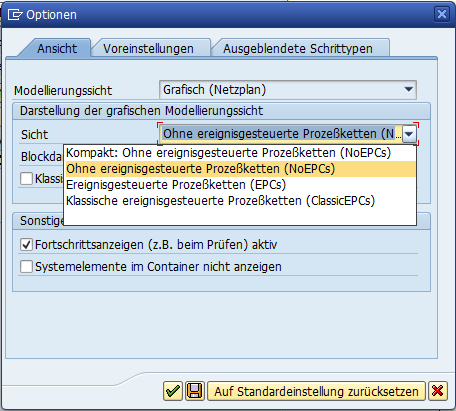
\includegraphics[width=300px]{grafiken/wf-builder_options-change-view.png}
	\caption{Ändern der Ansicht des Workflow Builders}
	\vspace{-10pt}
	\label{abb:workflow-change-view}
	\end{center}
\end{figure}

\subsection{Schritttypen}
\label{sec:builder-elemente}
% MARCO, STEFFEN
% tabelle mit elementen..
% was ist wofür gedacht
	\begin{longtable}{|c|p{2.5cm}|p{10.5cm}|}
		\hline
		\textbf{Symbol} & \textbf{Schritttyp} & \textbf{Beschreibung}\\
		\hline
		\includegraphicstotab[width=0.8cm]{grafiken/aktivitaet.png}
		& 
		Aktivität & Ausführen einer ABAP-Methode oder einer vordefinierten Aufgabe \\ 
		\hline \includegraphicstotab[width=0.8cm]{grafiken/web-aktivitaet.png} 
		& 
		Web-Aktivität & \gls{xml}-Dokument an eine URL senden, z.B. um Workflows in Fremdsystemen zu starten\\ 
		\hline 
		\includegraphicstotab[width=0.8cm]{grafiken/mail-versenden.png} 
		& 
		Mail-Versendung & Nachricht an Endnutzer versenden\\ 
		\hline 
		\includegraphicstotab[width=0.8cm]{grafiken/formular.png}
		& 
		Formular\-schritt & Anzeige von Daten und Möglichkeit zum Bearbeiten dieser durch Endnutzer\\ 
		\hline 
		\includegraphicstotab[width=0.8cm]{grafiken/benutzerentscheidung.png}
		& 
		Benutzer\-entscheidung & Beantworten einer Frage bzw. Treffen einer Entscheidung durch den Benutzer zur Beeinflussung des Workflows\\ 
		\hline 
		\includegraphicstotab[width=0.8cm]{grafiken/dokument-aus-vorlage.png}
		& 
		Dokument aus Vorlage & Anzeigen oder Bearbeiten von Dokumenten, die mit externen Anwendungen erstellt wurden mit Hilfe eines auf dem Rechner installierten Programms\\ 
		\hline 
		\includegraphicstotab[width=0.8cm]{grafiken/bedingung.png}
		& 
		Bedingung & Bedingte, selbstständige Entscheidung für einen Pfad aus zwei Möglichkeiten durch das System\\ 
		\hline 
		\includegraphicstotab[width=0.8cm]{grafiken/mehrfachbedingung.png}
		& 
		Mehrfach\-bedingung & Bedingte, selbstständige Entscheidung für einen Pfad aus mehreren Möglichkeiten durch das System\\ 
		\hline 
		\includegraphicstotab[width=0.8cm]{grafiken/ereigniserzeuger.png}
		& 
		Ereignis\-erzeuger & Auslösen eines Ereignisses, auf welches ein Warteschritt wartet\\ 
		\hline 
		\includegraphicstotab[width=0.8cm]{grafiken/warten.png}
		& 
		Warteschritt & Warten, bis ein durch einen Ereigniserzeuger generiertes Ereignis eintritt\\ 
		\hline 
		\includegraphicstotab[width=0.8cm]{grafiken/containeroperationen.png}
		& 
		Container\-operationen & Verändern von Elementen des Workflow-Containers (Umgebung des aktiven Workflows mit Variablen und Benutzerentscheidungen)\\ 
		\hline 
		\includegraphicstotab[width=0.8cm]{grafiken/ablaufsteuerung.png}
		& 
		Ablauf\-steuerung & Eingriff in den Ablauf des aktuellen Workflows - Abbruch oder Beenden einzelner Schritte oder des gesamten Workflows\\ 
		\hline 
		\includegraphicstotab[width=0.8cm]{grafiken/schleife.png}
		& 
		Schleifen & Mehrfache Ausführung eines Blocks von Schritten unter einer bestimmten Bedingung\\ 
		\hline 
		\includegraphicstotab[width=0.8cm]{grafiken/paralleler-abschnitt.png}
		& 
		Paralleler Abschnitt & Aufsplitten des Workflows in zwei parallel laufende Pfade\\ 
		\hline 
		\includegraphicstotab[width=0.8cm]{grafiken/ad-hoc-anker.png}
		& 
		Ad-hoc-Anker & Möglichkeit, einen anderen Workflow des Systems zu hinterlegen, der vom berechtigten Benutzer ausgeführt werden kann\\ 
		\hline 
		\includegraphicstotab[width=0.8cm]{grafiken/block.png}
		& 
		Block & Zusammenfassen mehrerer Schritte zu einem Block mit eigenen Variablen\\ 
		\hline 
		\includegraphicstotab[width=0.8cm]{grafiken/lokaler-workflow.png}
		& 
		Lokaler Workflow & Einfügen eines Sub-Workflows, welcher vollen Zugriff auf die Daten des aktuellen Workflows hat\\ 
		\hline 
		% Beschriftung festlegen:
		\caption{Symbolerklärung des \gls{sap} Workflow Builders}
		% ein Label definieren, mit dessen Hilfe man (an beliebiger Stelle im 	Dokument) Bezug nehmen kann:
		\label{tab:builderelemente}
\end{longtable}

%%%%%%%%%%%%%%%%%%%%%
%% KAPITEL HandsOn %%
%%%%%%%%%%%%%%%%%%%%%
%% MARCO
%%%%%%%%%%%%%%%%%%%%%
\section{Hands On}
In diesem Kapitel soll die Arbeit mit dem \gls{sap} Workflow Builder näher beleuchtet werden, indem zwei beispielhafte Prozesse zuerst in der Theorie erklärt und danach im System gebaut werden. Um eine Steigerung zu erreichen, wird die Kreation des ersten, sehr einfachen Workflows Schritt für Schritt beschrieben, wohingegen beim zweiten, etwas komplexeren Workflow darauf verzichtet wird, jede Eingabe zu erklären. Stattdessen wird dessen grobere Funktionsweise erläutert. 

\subsection{Erstes Beispiel: Kontrolle des Materials}
\label{sec:builder-1-bsp}
% kleiner sinnloser workflow (schleife,...) => aus dem Video Tutorial

\subsubsection{Vorstellung des Workflows}
\label{sec:builder-1-bsp-vorstellung}
Zum Einstieg soll ein Workflow angelegt werden, welcher einen sehr geringen Funktionsumfang hat. Dieser besteht aus folgenden Punkten:

\begin{itemize}
	\item Der Workflow soll automatisiert starten, sobald der Benutzer ein neues Material im System anlegt.
	\item Als erstes wird der Benutzer gefragt, ob er das soeben angelegte Material noch einmal kontrollieren will.
	\item Im Falle einer Entscheidung für "`ja"' wird das erzeugte Material angezeigt.
	\item Entscheidet sich der Benutzer gegen eine Anzeige des Materials, soll er darüber per E-Mail informiert werden.
\end{itemize}

Dieser Ablauf ergibt, gerade unter Betrachtung der Information per E-Mail darüber, dass das angelegte Material nicht angezeigt werden soll, nicht zwangsläufig einen Sinn, um ihn in einer existierenden Firma anzuwenden, soll aber stattdessen die Arbeit mit Startereignissen, Benutzerentscheidungen und weiteren Aktivitäten erklären.

\subsubsection{Umsetzung des Workflows}
\label{sec:builder-1-bsp-umsetzung}
Um den beschriebenen Workflow im Builder umzusetzen ist es sinnvoll, zuerst den Ablauf ohne Startereignis oder Datenübergabe zu erstellen. Zur Vereinfachung wird daher vorerst davon ausgegangen, dass bereits bekannt ist, um welches Material es geht, so wird nur von "`dem Material"' gesprochen. 

Als erstes soll der Benutzer gefragt werden, ob er das soeben erstellte Material anzeigen möchte. Dazu wird der Schritt \textit{Benutzerentscheidung} per \gls{dragdrop} auf das leere Feld zwischen dem schon vorhandenen Start- und Endereignis gezogen. Daraufhin öffnet sich das Formular zur Konfiguration der Abfrage. Als Text soll hier beispielsweise eingegeben werden "`Wollen Sie das Material anzeigen?"'. Als mögliche Entscheidungsalternativen sollen in der unteren Hälfte des Formulars "`Ja, ich will"' und "`Nein, danke"' mit den zugehörigen Ausgangsbezeichnungen "`ja"' und "`nein"' angegeben werden. Der Bearbeiter der Abfrage soll der Workflow Initiator sein. Hierzu wird im Menü unter "`Bearbeiter"' der entsprechende Ausdruck eingefügt. (Abbildung \ref{abb:workflow-bsp1-benentsch_form}) Dies ist die Person, welche den Workflow gestartet hat. Der Bearbeiter ist die Person, welche später die Abfrage per E-Mail erhält.

\begin{figure}[h]
	\begin{center}
	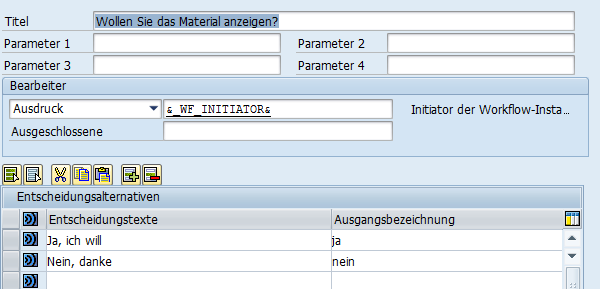
\includegraphics[width=400px]{grafiken/wf-builder_bsp1_formular-benutzerentscheidung.png}
	\caption{Ausgefülltes Formular zur Benutzerentscheidung}
	\vspace{-10pt}
	\label{abb:workflow-bsp1-benentsch_form}
	\end{center}
\end{figure}

Nachdem die Benutzerentscheidung eingefügt wurde, teilt das System den bisher linearen Pfad in zwei Teile, die mit den angegebenen Kurztexten der Antwortmöglichkeiten versehen sind. Da der Benutzer im Falle einer Entscheidung für "`nein"' eine E-Mail erhalten soll, wird nun der Schritt \textit{Mail versenden} auf den entsprechenden Pfad gezogen. Im nun folgenden Eingabefeld muss nur der Text und der Betreff der Mail ausgefüllt werden. Wird als Empfängerart "`Organisationsobjekt"' und wieder der Workflow Initiator ausgewählt, so wird die Nachricht innerhalb des \gls{sap} Systems versendet. (Abbildung \ref{abb:workflow-bsp1-mail_form})

\begin{figure}[h]
	\begin{center}
	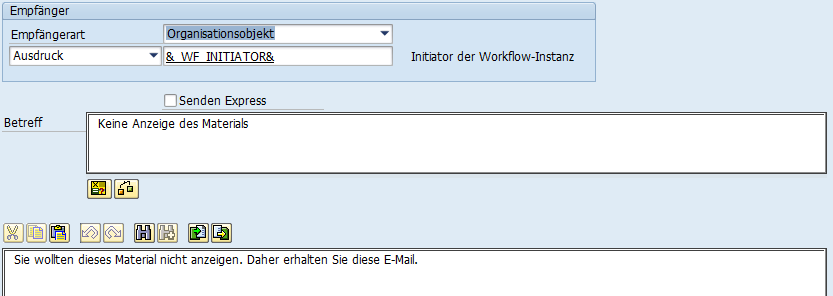
\includegraphics[width=400px]{grafiken/wf-builder_bsp1_formular-mail.png}
	\caption{Das ausgefüllte Formular zur internen Mail}
	\vspace{-10pt}
	\label{abb:workflow-bsp1-mail_form}
	\end{center}
\end{figure}

Der letzte noch fehlende Punkt im Prozess ist die eigentliche Anzeige des Materials. Hierzu wird der Schritt \textit{Aktivität} auf den noch verbleibenden, leeren Pfad nach der Benutzerentscheidung gezogen. Die Konfiguration dieses Schrittes ist etwas aufwändiger, da für jede Aktivität, sofern noch nicht vorhanden, eine Aufgabe angelegt werden muss. Dies kann erledigt werden, indem das Menü neben dem Schriftzug "`Aufgabe"' geöffnet und der Eintrag "`Aufgabe anlegen"' ausgewählt wird. Im nun angezeigten Formular (Abbildung \ref{abb:workflow-bsp1-aufgaben_form}) muss der neuen Aufgabe nun ein Kürzel und eine Bezeichnung zugewiesen werden. Da es im \gls{sap} System den vorgefertigten \gls{bor} Objekttypen "`Standard Material"' gibt, ist es für den Benutzer nicht von Nöten, eine eigene \gls{abap} Klasse hierfür zu erstellen. Als Objektkategorie kann "`\gls{bor}-Objekttyp"' ausgewählt und als Objekttyp \\texttt{BUS1001006} eingegeben werden. Ist der Objekttyp nicht bekannt, kann hier die im \gls{sap} System global verfügbare Eingabehilfe verwendet werden. Mit dieser kann danach auch aus den verfügbaren Methoden des Objekttypen gewählt werden. Im konkreten Fall wird die Methode \texttt{DISPLAY} verwendet.

\begin{figure}[h]
	\begin{center}
	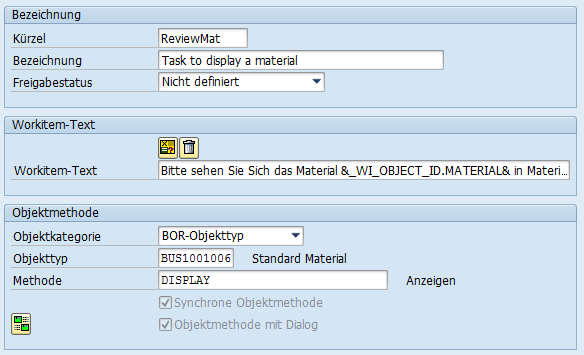
\includegraphics[width=400px]{grafiken/wf-builder_bsp1_formular-aufgabe.png}
	\caption{Ausgefülltes Formular zur neuen Aufgabe}
	\vspace{-10pt}
	\label{abb:workflow-bsp1-aufgaben_form}
	\end{center}
\end{figure}

Letztlich sollte im Feld \textit{Workitem-Text} noch ein Text angegeben werden, der dem Endnutzer beschreibt, was zu erledigen ist. Mit dem entsprechenden Button 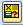
\includegraphics[height=1em]{grafiken/wf-builder_bsp1_formular-aufgabe_btn_eingabehilfe-ausdruck.png} links neben dem Papierkorb über dem Eingabefeld können hierzu Variablen aus einer zusätzlichen Eingabehilfe (Abbildung \ref{abb:workflow-bsp1-aufgaben_form-inputhelp}) eingefügt werden.

Nach dem Speichern der Aufgabe aber vor dem Schließen des Aufgabeneditors sollte noch eine letzte Option getroffen werden. Diese definiert die Aufgabe als generelle Aufgabe, was bedeutet, sie kann von jedem Benutzer des Systems ausgeführt werden. Die Pflege des Bearbeiters erfolgt über das Menü in der Titelleiste des \gls{sap} Programms. Hierzu wird das Menü \textit{Zusatzdaten} - \textit{Bearbeiterzuordnung} - \textit{Pflegen} aufgerufen und nach einem Klick auf \textit{Eigenschaften...} die Auswahl "`Generelle Aufgabe"' getroffen. Über den normalen zurück-Button des Systems kann nun zum Bearbeiten der Aktivität zurück gesprungen werden. Dort ist, wie bei den vorigen Elementen auch, als Bearbeiter der Workflow Initiator einzustellen. 

Sind sämtliche Einstellungen getroffen und es wird wieder das Hauptfenster inklusive des Workflows angezeigt, so muss als letzte Einstellung noch dafür gesorgt werden, dass das Objekt "`Material"' beim Starten des Workflows importiert wird. Dies ist nötig, da das Objekt nicht im Laufe des Prozesses generiert wird, sondern dieser gestartet wird, nachdem ein Material angelegt wurde. Um diese Änderung durchzuführen, muss der Benutzer, wie in Kapitel \ref{sec:win-overview-alternative} beschrieben, zur Ansicht der Workflow-Container wechseln, den oben beschriebenen Container "`BUS1001006"' mit einem Doppelklick öffnen und dort im Reiter \textit{Eigenschaften} das Kästchen vor "`Import"' anhaken (Abbildung \ref{abb:workflow-bsp1-containeredit-import} des Anhangs).

Nach diesem Schritt, nachdem er gespeichert 
\includegraphics[height=1em]{grafiken/btn_sap_save.png}, geprüft 
\includegraphics[height=1em]{grafiken/btn_sap_check.png} und aktiviert 
\includegraphics[height=1em]{grafiken/btn_sap_activate.png} wurde, kann de Workflow in der Testumgebung des Builders zum ersten Mal ausgeführt 
\includegraphics[height=1em]{grafiken/btn_sap_excecute.png} werden. 

Nun sind von den in Kapitel \ref{sec:builder-1-bsp-vorstellung} genannten Punkten alle bis auf den ersten umgesetzt. Um den Prozess automatisiert zu starten, sobald ein neues Material angelegt wird, benötigt der Workflow ein sogenanntes \textit{Startereignis}. Diese können in einem Formular gepflegt werden, welches über das Kontextmenü \textit{Springen} - \textit{Grunddaten} unter dem Reiter \textit{Startereignisse} erreichbar ist. Um ein neues Startereignis anzulegen sind die folgenden Einstellungen zu treffen:

\begin{itemize}
	\item In der Spalte \textbf{Kategorie} muss festgelegt werden, dass es sich um ein \gls{bor}-Objekt handelt. 
	\item Naheliegenderweise muss in der Spalte \textbf{Objekttyp} der bereits bekannte Typ \texttt{BUS1001006} angegeben werden.
	\item Das auszuwählende \textbf{Ereignis des Objekts} ist \texttt{CREATED}.
	\item Über einen Klick auf den linken der drei gelben Buttons muss das Ereignis \textbf{aktiviert} werden.
	\item Letztlich muss der \textbf{Datenfluss} über den mittleren Button 
\includegraphics[height=1em]{grafiken/wf-builder_bsp1_btn-datenfluss.png} und einem Druck auf den grünen Haken 
\includegraphics[height=1em]{grafiken/btn_sap_apply.png} aktiviert werden, sodass beim Erstellen eines Materials die Materialnummer an den Workflow Container übergeben wird.
\end{itemize}

Der erstelle Workflow ist nun nach einer weiteren Aktivierung (siehe oben) der getroffen Definition fertiggestellt und kann verwendet werden. Er sollte vom System, wie in Abbildung \ref{abb:workflow-bsp1-complete} gezeigt, dargestellt werden und startet sich nun automatisch, sobald über die \gls{transaktion} \texttt{MM01} ein Material angelegt wird. Den Workflow erhält der entsprechende Benutzer standardmäßig in seinen \gls{businessworkplace} ausgeliefert, sodass er diesen dort starten kann.

\subsection{Zweites Beispiel: Erstellung und Genehmigung einer Abwesenheitsnachricht}
\label{sec:builder-2-bsp}
% demo workflow aus den vorlagen nehmen (abwesenheitsbestätigung)

\subsubsection{Vorstellung des Workflows}
\label{sec:builder-2-bsp-vorstellung}
% wofür ist der workflow gut, was soll er tun (aus anwendersicht)
Als zweites, etwas komplexeres Beispiel soll der Prozess der Abwesenheitsnachricht dienen. In diesem Prozess erstellt der Angestellte einer Firma direkt nach dem Start des Workflows eine Abwesenheitsmitteilung mit Hilfe eines vorgegebenen Formulars. Daraufhin erhält der Vorgesetzte des Angestellten eine Mitteilung in sein internes Postfach, welche den Hinweis enthält, dass er die Mitteilung bearbeiten soll. Hiernach soll es zwei Möglichkeiten geben. Erfolgt eine Genehmigung, soll der Antragsteller benachrichtigt werden. Im Falle einer Ablehnung muss der Workflow Initiator die Wahl haben, die Mitteilung zu überarbeiten oder zu löschen. Im Falle einer Überarbeitung muss der Prozess ab der Genehmigung erneut beginnen.

\subsubsection{Umsetzung des Workflows}
\label{sec:builder-2-bsp-umsetzung}
% technische sicht, "`klickbares"' howto
Nachdem in Kapitel \ref{sec:builder-1-bsp-umsetzung} die Umsetzung sehr genau beschrieben wurde und die Konfiguration einzelner Aktivitäten und Benutzerentscheidungen bekannt ist, soll dieser Prozess nun vom logischen Ablauf her betrachtet werden und die entsprechende Umsetzung im \gls{sap} System aufgezeigt werden.

Die Idee hinter der Logik dieses Workflows ist ein sogenanntes Flag, welches eine Art Variable darstellt, welche durch zwei verschiedene Zustände aufzeigt, ob die Bearbeitung der Abwesenheitsmitteilung abgeschlossen ist oder die Bearbeitungsschleife erneut durchlaufen werden muss. Dieses Flag wird im schon bekannten \textit{Workflow Container} angelegt und ist eine \gls{abap}-Dictionary-Referenz des Feldes \texttt{RETURNCODE} der Struktur \texttt{SWD\_LINES}. Die Konfiguration des Containerelements kann in Abbildung \ref{abb:workflow-bsp2-container-flag} eingesehen werden. Ein zusätzliches Container-Element ist das eigentliche Formular zur Anzeige und Bearbeitung einer Abwesenheitsmitteilung. Dieses Formular ist ein im System standardmäßig vorhandener \gls{bor} Objekttyp mit dem Namen \texttt{FORMABSENC} und kann somit einfach angelegt werden (Abbildung \ref{abb:workflow-bsp2-container-form}). 

Nachdem die beiden benötigten Elemente des Containers angelegt wurden und somit das nötige Umfeld steht, kann nun der eigentliche Workflow erstellt werden. Zum einfachen Nachbau des Prozesses ist die Konfiguration der einzelnen Aufgaben jeweils im Anhang abgebildet. 

Wie bereits in Kapitel \ref{sec:builder-2-bsp-vorstellung} erwähnt, soll nach dem Start des Workflows eine Abwesenheitsmitteilung angelegt werden. Dies wird durch eine entsprechend konfigurierte Aktivität erreicht, wobei die benötigte Aufgabe bereits im System unter dem Kürzel \texttt{exformabscre} vorhanden ist und der Bearbeiter der Workflow Initiator ist. Als Schrittbezeichnung wählen wir \textit{AM anlegen}. (Abbildung \ref{abb:workflow-bsp2-act_am-anlegen})

Der noch folgende Rest des Prozesses soll, wie in Kapitel \ref{sec:builder-2-bsp-vorstellung} beschrieben, komplett wiederholt werden, sofern der Benutzer sich später für die erneute Überarbeitung der Mitteilung entscheidet. Daher wird nun eine Schleife eingefügt, sodass sämtliche noch folgenden Schritte direkt in diese eingebaut werden können. Dies verhindert späteres Umbauen des Workflows beim nachträglichen Einfügen der Schleife. Wurde die benötigte \textit{Schleife (Until)} am entsprechenden Platz im Prozess eingefügt, so öffnet sich das Konfigurationsfenster derselben. Die Bedingung kann, da das benötigte Flag bereits erstellt wurde, mit Hilfe einfach mit der entsprechenden Eingabehilfe (Abbildung \ref{abb:workflow-bsp2-act_loop_inputhelp}) eingefügt werden. Die komplette Konfiguration der Schleife kann in Abbildung \ref{abb:workflow-bsp2-act_loop} eingesehen werden.

Anhand der nächsten Aktivität zur Genehmigung oder Ablehnung der Abwesenheit wird klar, dass eine Aktivität, je nach Konfiguration der entsprechenden Aufgabe dahinter, mehr als einen Ausgang haben kann. Nachdem die Aufgabe eingetragen wurde, bleibt noch die Konfiguration des Bearbeiters. Da die Genehmigung dem Vorgesetzten obliegt, kann hier nicht, wie gewohnt, der Workflow Initiator eingetragen werden. Da die Person, welche die Aufgabe bearbeiten soll beim Erstellen des Prozesses noch nicht bekannt ist, sondern vom Workflow Initiator abhängt, wird aus dem Menü unter Bearbeiter der Wert \textit{Regel} ausgewählt und die im System unter dem Kürzel \texttt{saf\_manager} vorhandene Regel zum finden eines Vorgesetzten in das Textfeld dahinter eingetragen. (Abbildung \ref{abb:workflow-bsp2-act_am-genehmigen_klein}) Die Konfiguration der kompletten Aufgabe ist in Abbildung \ref{abb:workflow-bsp2-act_am-genehmigen} einsehbar.

\begin{figure}[h]
	\begin{center}
	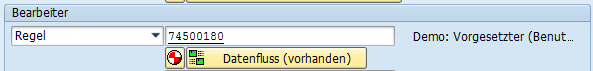
\includegraphics[width=1.0\textwidth]{grafiken/wf-builder_bsp2_act_am-genehmigen_klein.png}
	\caption{Verwenden der Regel zum Auswählen des Vorgesetzten}
	\vspace{-10pt}
	\label{abb:workflow-bsp2-act_am-genehmigen_klein}
	\end{center}
\end{figure}

Dem Pfad \textbf{genehmigt} nach der letzten Aufgabe soll ein Schritt eingefügt werden, der das oben erwähnte Flag so setzt, dass die Ausführung des Prozesses von der eingebundenen Schleife nicht wiederholt wird. Dieser Schritt kann einfach über den Schritttypen \textit{Containeroperation} erledigt werden, indem das \textit{Ergebniselement} mit Hilfe der entsprechenden Zuweisung auf den Ausdruck \texttt{000} gesetzt wird (Abbildung \ref{abb:workflow-bsp2-act_flag-0000}). Anschließend soll das System automatisiert mit Hilfe der entsprechenden Aufgabe (Abbildung \ref{abb:workflow-bsp2-act_message-genehmigt}) eine Benachrichtigung über die Genehmigung versenden.

\begin{figure}[h]
	\begin{center}
	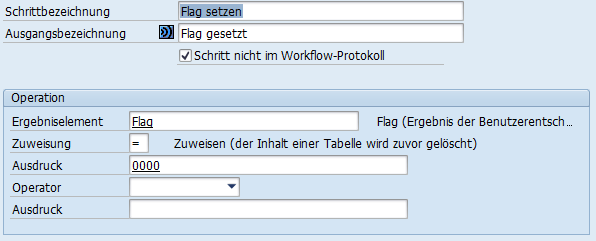
\includegraphics[width=0.75\textwidth]{grafiken/wf-builder_bsp2_act_flag_0000.png}
	\caption{Setzen des Flags auf den Wert 0}
	\vspace{-10pt}
	\label{abb:workflow-bsp2-act_flag-0000}
	\end{center}
\end{figure}

Nachdem der erste Pfad nun vollständig mit den nötigen Schritten befüllt wurde, soll der Workflow Initiator nun im Pfad \textbf{abgelehnt} danach gefragt werden, wie er weiter vorgehen möchte. Die gegebenen Möglichkeiten sind das Löschen oder das Überarbeiten der Abwesenheitsmitteilung. Da diese Entscheidung zwar den weiteren Verlauf des Prozesses beeinflusst, allerdings nicht, wie die Genehmigung, in einer Datenbank festgehalten werden muss, kann dieser Schritt durch eine simple \textit{Benutzerentscheidung} gelöst werden. Innerhalb dieser Entscheidung kann zur besseren Übersicht im Titel der Abfrage die Nummer der Abwesenheitsmitteilung angegeben werden. Dies erfolgt durch ein kaufmännisches Und als Platzhalter und dem Eintragen des entsprechenden Parameters in die Parameterliste darunter. Die entsprechende Konfiguration, die ähnlich schon in Kapitel \ref{sec:builder-1-bsp-umsetzung} erklärt wurde, kann in Abbildung \ref{abb:workflow-bsp2-act_was-tun} eingesehen werden. Auch nach dieser Entscheidung teilt das System den Pfad wieder in zwei weitere Pfade auf, welche wie folgt konfiguriert werden.

Der Pfad \textbf{löschen} wird mit einer Aktivität und der entsprechenden Aufgabe \texttt{AF\_delete} zum Löschen einer Mitteilung (Abbildung \ref{abb:workflow-bsp2-act_am-loeschen}) und der Containeroperation zum Setzen des Flags, wie in Abbildung \ref{abb:workflow-bsp2-act_flag-0000} gefüllt. Wird der Pfad \textbf{überarbeiten} eingeschlagen, so ist ein Setzen des Flags nicht nötig, da der Workflow ein weiteres Mal durchlaufen werden muss. Der Benutzer soll allerdings davor mit Hilfe einer Aktivität und der Aufgabe \texttt{AF\_update} die Möglichkeit erhalten, seine Mitteilung zu bearbeiten. (Abbildung \ref{abb:workflow-bsp2-act_am-editieren})

%%%%%%%%%%%%%%%%%%%%%%%%%%
%% KAPITEL Fremdsysteme %%
%%%%%%%%%%%%%%%%%%%%%%%%%%
%% JONAS 
%%%%%%%%%%%%%%%%%%%%%%%%%%
\section{Schnittstellen}

\subsection{SAP Fremdsysteme}
\label{sec:export-sap}

\gls{sap} Systeme liefern Workflows, die auf das Ziel der Applikation ausgelegt sind. \gls{erp}, \gls{crm} und \gls{srm} sind Beispiele für Systeme, die eingebaute, vordefinierte Workflows bereitstellen. 

Die Workflows sind anpassbar, um den Bedürfnissen der Firma gerecht zu werden. Es können mit dem Workflow Builder ganz eigene Geschäftsprozesse entwickelt werden, die natürlich über Modulgrenzen hinweg Zugriff auf Daten besitzen. So können Daten aus einem \gls{crm}-System in einem \gls{erp} zur Analyse, Auswertung und Bearbeitung von Daten hinzugezogen werden.

\subsection{XML}
\label{sec:export-xml}
% was ist dieses Format
% in welche Programme kann man es importieren?

\gls{xml} ist die Abkürzung für E\textbf{x}tensible \textbf{M}arkup \textbf{L}anguage und bezeichnet eine Auszeichnungssprache. Mit dieser können hierarchisch strukturierte Daten in Textform dargestellt werden. \gls{xml} besteht aus Elementen, deren Name, bis auf ein paar Ausnahmen, frei gewählt werden darf. Elemente haben einen Anfangs- ($\langle$elementName$\rangle$) und einen Endtag ($\langle$/elementName$\rangle$). Zwischen den Tags können weiter Elemente, Text und Knoten stehen. Diese sind dem Element dann untergeordnet.

Das World Wide Web Consortium, kurz \gls{w3c}, hat \gls{xml} als eine Metasprache definiert, auf deren Basis anwendungsspezifische Auszeichnungssprachen entwickelt werden können. Diese werden beschrieben durch ein Schema, welches festlegt, welche Elemente verwendet werden dürfen und welches Verhalten diese aufweisen \cite{XML}. So ist \gls{zb} auch XHTML definiert.

\subsection{BPMN und BPML}
\label{sec:export-bpmn-bpml}
% was ist dieses Format
% in welche Programme kann man es importieren?

\textbf{B}usiness \textbf{P}rocess \textbf{M}odel and \textbf{N}otation (\gls{bpmn}) ist eine grafische Spezifikationssprache, welche Symbole bereitstellt mit deren Hilfe Geschäftsprozesse und Arbeitsabläufe dargestellt werden können \cite{BPMN}. \gls{bpmn} wurde 2005 von der \gls{omg}, auch zuständig für \gls{zb} \gls{uml}, übernommen und gewann ab dann an Bedeutung in der Informatik. Außerdem wurde sie 2013 zum internationalen Standard (ISO/IEC 19510:2013) erhoben \cite{OMG}.

Da sich \gls{bpmn} rein auf die Darstellung von Workflows bezieht wurden mehrere, von \gls{xml} abgeleitete, Auszeichnungssprachen entwickelt, um Business Process Models auch als, für einen Computer verständliche, Daten aufschreiben zu können. Dazu zählen \gls{zb} \gls{bpel}, \gls{xpdl} oder \gls{bpml} \cite{BPMN}.

Die \textbf{B}usiness \textbf{P}rocess \textbf{M}odeling \textbf{L}anguage (\gls{bpml}) wird von \gls{sap} im Workflowbuilder (\ref{chap:builder}) verwendet um Geschäftsprozesse zu exportieren. Da \gls{bpml} auch unter dem Dach der \gls{omg} steht wird sie auch in anderen Workflow Management Systemen, wie \gls{zb} jBPM, Camunda BMP oder ARIS, verwendet. Dadurch lassen sich \gls{sap}-interne Geschäftsprozesse auch extern einbetten \cite{BPML}.